\documentclass[../thesis_seyed.tex]{subfiles}
% \graphicspath{{\subfix{../img/}}}
\begin{document}
\chapter{GROUP-LEVEL CORTICOMUSCULAR CONNECTIVITY DURING SEATED LOCOMOTOR PERTURBATIONS FOR YOUNG AND OLDER ADULTS}
\section{Introduction}

Motor and locomotor perturbations elicit cortical and muscular activity, potentially reducing motor errors. Several cortical and subcortical brain areas are known to engage in monitoring motor errors. The anterior cingulate cortex in the mid-prefrontal brain region is likely to detect motor errors with sensory inputs and the expected goal \cite{Holroyd2002-fl}. The supplementary motor area integrates neural pathways from the motor cortex and anterior cingulate and likely acts as a sensory and executive hub for processing errors \cite{Peterson2019-wz}. The posterior parietal cortex likely processes the differences between the visual and sensorimotor inputs \cite{Peterson2018-ht}. Nevertheless, the activities of these brain areas are not essentially exclusive. For example, the left posterior parietal cortex has a critical role in joint impedance control, while the right prefrontal cortex controls the limb speed during perturbed upper limb motor tasks \cite{Mutha2014-ea}. Perturbations tend to increase muscular activation and agonist/antagonist co-contraction \cite{Huang2014-to,Thoroughman1999-pz}. Not surprisingly, the cortico-cortical, intra-muscular, and corticomuscular coherence also increases with perturbations indicting increased cortical control over muscular activation \cite{Sato2019-qb,Zandvoort2019-xl,Gentili2015-pq}.

The age-related differences in cortical and muscular activity are in different directions. Older adults implement more co-contraction in response to motor perturbations and would likely reduce their contraction less than young adults as they gain more experience with the perturbations \cite{Huang2014-nh}. However, locomotor perturbation studies also indicated that older adults use simpler muscular control through fewer muscle synergies or fewer driving muscles to maintain similar motor performance as young adults \cite{Allen2018-kd,Da_Silva_Costa2020-vl}. Many studies have indicated “overactivation” of older adults’ brain regions compared to young adults as a compensatory mechanism for similar motor performance \cite{Reuter-Lorenz2008-bn,Seidler2010-yv}. Such overactivation would increase connectivity at both cortical and muscular levels when facing motor challenges \cite{Walker2020-kh,Johnson2012-fv,Kamp2013-ga}. In contrast, a couple of studies on standing and locomotor tasks using channel EEG and EMG signals indicated weaker connectivity in older adults \cite{Roeder2020-tv,Ozdemir2018-yp,Yoshida2017-un}. The different methods for connectivity computation, lack of source-resolved EEG, and inter-subject variability may contribute to the different outcomes observed in the connectivity studies \cite{Clark2019-iv,Holler2017-ac}.

Nevertheless, the decrease in cortico-muscular connectivity due to neurological impairments is well-documented \cite{Yokoyama2020-ie,Larsen2017-ya,Chen2018-ns}, and rehabilitation can improve the connectivity levels or use connectivity as a metric for motor improvement \cite{Youssofzadeh2016-sl,Chowdhury2020-qa}. We previously introduced perturbed recumbent stepping as a locomotor task that can elicit similar brain dynamics as perturbed walking, especially in the anterior cingulate cortex and supplementary motor areas \cite{Shirazi2021-ha}. We also showed that older adults recruited fewer muscle-pairs than young adults to perform perturbed stepping, despite having similar motor errors as young adults. The main advantage of recumbent stepping and other seated exercises is that subjects would not require to maintain their balance while performing the exercise, which is especially beneficial for accessible walking rehabilitation. Determining the connectivity markers of perturbed stepping will set the baselines for using this exercise as a rehabilitation approach to improve corticomuscular connectivity.

The purpose of this study was to quantify the corticomuscular connectivity patterns of young and older adults in response to brief perturbations during recumbent stepping. We also aimed to determine whether the timing of the perturbations modulated corticomuscular connectivity. We hypothesized that the corticomuscular connectivity would increase around the perturbation timing, especially between the motor cortex and the driving muscles, namely, posterior deltoids and rectus femoris. This hypothesis was based on our previous EEG and EMG analyses showing increased electrocortical and muscular activation around the stepping perturbation \cite{Shirazi2021-ha}. We also hypothesized that the anterior cingulate cortex would have increased direct causal connectivity from a subset of muscles around the perturbation timing, which would act as sensory feedback for error monitoring. In this study, we use connectivity and causal relation or effect interchangeably.

\section{Methods}

Seventeen adults (11 females, age 25  4.9 years) and 11 older adults (4 females, age 68  3.6 years) participated in the study. Subjects were all right-handed as they would pick an object from the floor, and they reported no prior neurological or physical problems for two years prior to their test.  The Institutional Review Board of the University of Central Florida approved the study, and subjects gave their written informed consent before starting the experiment.

\subsection{Hardware}
We used a recumbent stepper integrated with a servomotor \cite{Huang2009-of} to introduce brief perturbations in the form of added resistance during stepping. The stepper was mechanically coupled in a way that the contralateral arm and leg would extend together. We used the servomotor to briefly increase stepping resistance for 200 ms as the subject's left or right leg was at the extension-onset or mid-extension. The increased stepping resistance was a torque-controlled algorithm that would require 3x the normal torque to drive the stepper at 60 steps per minute. We used the servomotor's position sensor to record the stepper's kinematics at 100Hz.

We used twelve wireless electromyography, EMG, sensors (Trigno, Delsys, Natick, MA) to collect muscular activity at \td1.1 kHz. We attached the EMG sensors on the tibialis anterior, soleus, rectus femoris, semitendinosus, anterior deltoid, and posterior deltoid on both left and right sides (Hermens et al. 1999). Here, we only analyzed the left-side muscles because our preliminary results indicated that including all muscles would decrease the connectivity accuracy. We used high-density electroencephalography, EEG, system (ActiveTwo, 128 electrodes, BioSemi B.V., Amsterdam, the Netherlands) to collect brain activities at 512 Hz. We placed the EEG cap and electrodes according to the BioSemi manual and used a 3D scanner (Structure I, Occipital Inc., CO) to record the electrode's 3D locations \cite{Shirazi2019-im}. Data streams of the different systems were synchronized using a trigger signal from the stepper controller to the EMG and EEG systems.

\subsection{Protocol}
Data collection consisted of four 10-minutes stepping tasks; each task only included one perturbation type at the mid-extension or extension-onset of the left or right legs. Each task started and ended with two-minutes pre and post unperturbed stepping blocks and included a six-minute-long perturbation block, in which subjects would experience perturbation at each stride. There was also a random one-in-five catch stride in the perturbation block, which did not include perturbations. Before starting each task, we asked subjects to 1) follow the visual pacing cue presented in front of them at 60 steps per minute, 2) step smoothly as they were walking, and 3) use both arms and legs to drive the stepper. A complete explanation of the protocol has been presented previously \cite{Shirazi2021-ha}. We determined the stepping events using the kinematic information from the stepper servomotor. Each stride was from the start of the perturbed-leg extension to the next perturbed-leg extension. Perturbation events were the start of the increased stepping resistance for each stride.

\subsection{EEG processing}
EEG and EMG data were processed and analyzed in MATLAB environment (R2018b, MathWorks Inc., Natick, MA) with a custom pipeline based on EEGLAB version 2019.0 \cite{Delorme2004-yy} (Figure \ref{fig:connProcc}). The EEG pre-processing pipeline is largely similar to our previous study on young adults' perturbed stepping \cite{Shirazi2021-ha}. In summary, we used a high-pass filter at 1 Hz and a 60 Hz line-noise filter to clean the EEG data before applying the template correlation rejection method to identify the channels that had a high correlation to the stepping events \cite{Oliveira2017-pk}. We then used step-wise channel and frame rejection to create 32 datasets for each subject with a range of conservative to lenient noise rejection. The signal noise rejection metrics were range, variance, kurtosis, and correlation to other channels \cite{Bigdely-Shamlo2015-ow}. The frame noise rejection metric was the EEG inter-quartile variability to the overall median of the signal during each task. We used adaptive mixture independent component analysis (AMICA) to quantify the independent components (ICs) for each of the 32 datasets, estimated the IC locations in the brain using DIPTFIT, and used a multivariate classifier (ICLabel) to estimate the number of "brain" ICs for each dataset \cite{Palmer2008-jx,Pion-Tonachini2019-gv}. We ultimately the dataset with the most "brain" ICs at the representative dataset for each subject.

\begin{figure}[tb]
    \centering
    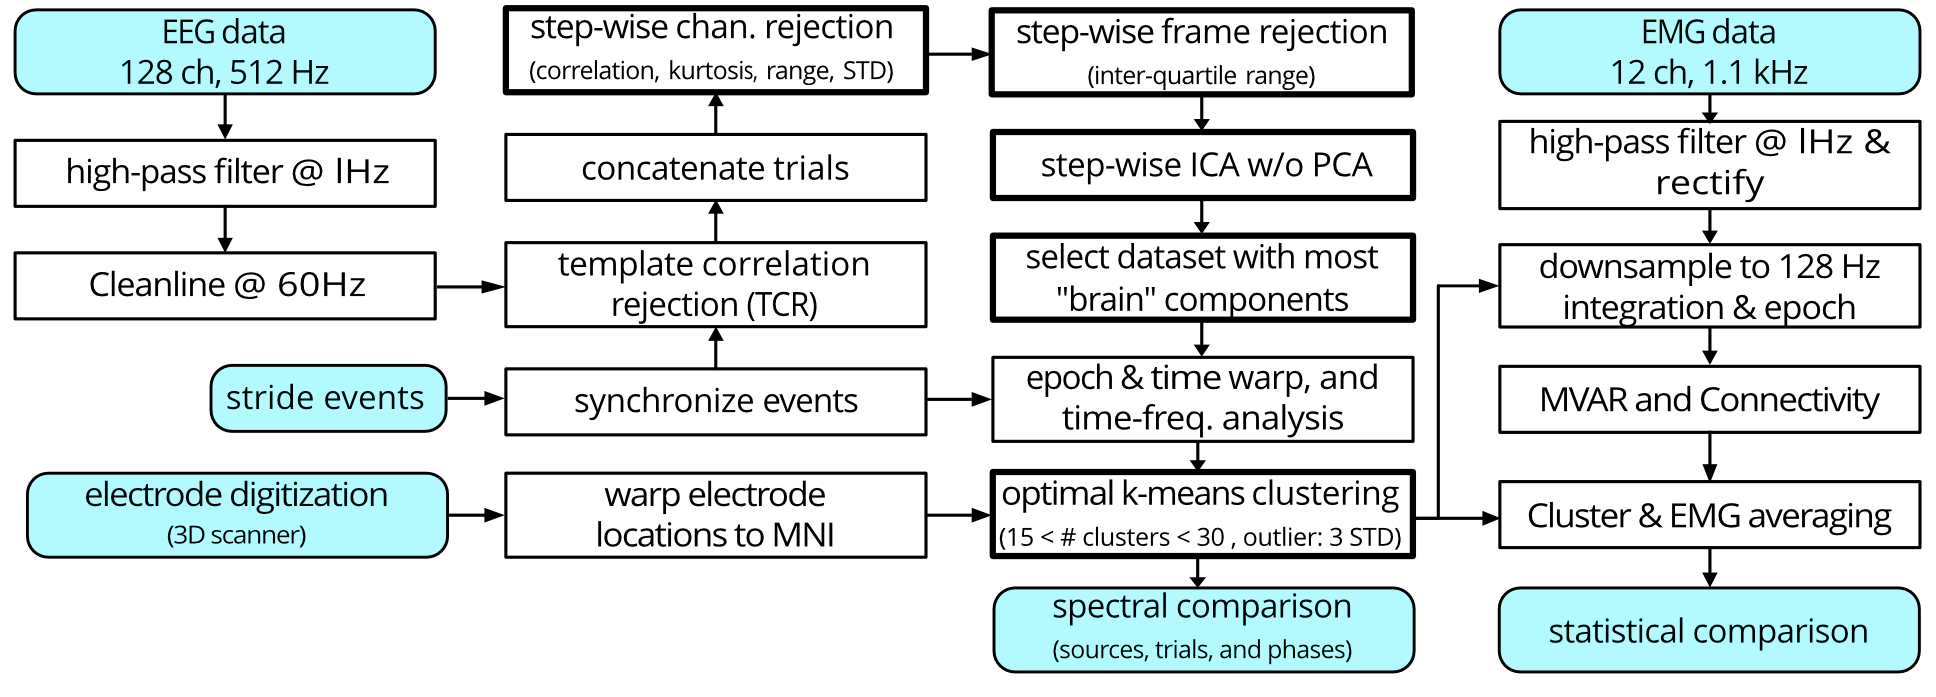
\includegraphics[width=\linewidth]{../img/figure 1 - workflow.jpg}
    \caption{EEG and connectivity processing pipelines. The strong boxes indicate novel methods designed in this research. The shaded boxes indicate input or output.}
    \label{fig:connProcc}
\end{figure}

We clustered ICs from young and older adults separately based on the IC location, power spectrum, and scalp map. We used the 3 to 25 Hz range for power spectrum and the Laplacian of the scalp map to perform the clustering \cite{Hjorth1975-ea}. We used optimal k-means clustering to select the number of cortical clusters for young and older adults separately and focused on the clusters that included >70\% of the subjects. If the ICs in a cluster were mostly in a Brodmann area, we would assign that cluster with that Brodmann area \cite{Lancaster2000-aj,Shirazi2019-im}. If a cluster spanned across multiple Brodmann areas, we would attribute the cluster with the region that would encompass the cluster's ICs.

Finally, we computed the temporal profile of the spectral power of each cluster, commonly known as the event-related spectral perturbations (ERSP) \cite{Makeig1993-jx}. We epoched the EEG data from -400 ms to +400 ms of the perturbation events. We baseline normalized the spectral power using the average spectral power during pre and computed the statistically significant event-related synchronization and desynchronization for the ERSPs using EEGLAB permutation functions with alpha equal 0.05 \cite{Pfurtscheller1999-oi}. ERPS images only show significant spectral fluctuations.

\subsection{Connectivity processing}
We used the cortical source clusters and EMG from twelve upper and lower limb muscles to compute connectivity metrics mainly based on Peterson and Ferris's group-level connectivity analysis of balance-beam walking and standing perturbations \cite{Peterson2019-wz} (Figure \ref{fig:connProcc}).  We selected each subject's ICs that contributed to the cortical clusters and added the EMG signals after high-pass filtering at 1 Hz and rectifying \cite{Myers2003-dv}. We epoched the integrated IC and EMG data from -2 sec to +2 sec of the perturbation events to provide the required data for estimating the multivariate autoregressive models for each subject. We used the Viera-Morf algorithm with 1.3-sec window size and 0.01-sec window step-size to fit a multivariate autoregressive model with an order equal to 32 to each subject's integrated dataset \cite{Marple1989-wh,Cohen2014-vt}. We used the 1.3-sec window size to improve the model fit and the 0.01-sec window step-size to provide 10 ms temporal resolution for the connectivity analysis. The model order of 32 provides a spectral resolution of 4 Hz for the connectivity analysis and lets the autoregressive model take more of the past data into the model. The higher model orders, up to 40, have not shown significant noise increases inherent to estimating a greater number of variables in a similar study \cite{Peterson2019-wz}.

We used the direct Directed transfer function (dDTF) to estimate the direction connectivity between cortical ICs and EMG signals. The main advantages of dDTF are the casual directionality and the separation of direct causal effects from indirect causal effects \cite{Korzeniewska2003-ol,Peterson2019-wz,Cohen2014-vt,Kaminski2001-oi}. Casual directionality provides the source and target of the "information flow" instead of the mere coherent activation of two sources \cite{Kaminski2001-oi}. Exclusion of the hierarchy effect where a source upstream has a causal effect on all downstream targets is another advantage of dDTF because only the direct causal influences are taken into account \cite{Korzeniewska2003-ol}. A phantom-head study with motion artifacts also had shown that dDTF could effectively recover the casual relations between signal sources \cite{Peterson2018-la}. We finally averaged the cortical clusters and EMG source connectivity results across subjects, baseline normalized to the average connectivity from -400 ms to -100 ms seconds and showed the significant increases and decreases in connectivity similar to the ERSP plots from -400 ms to +400 ms of the perturbation event.

\begin{figure}[tb]
    \centering
    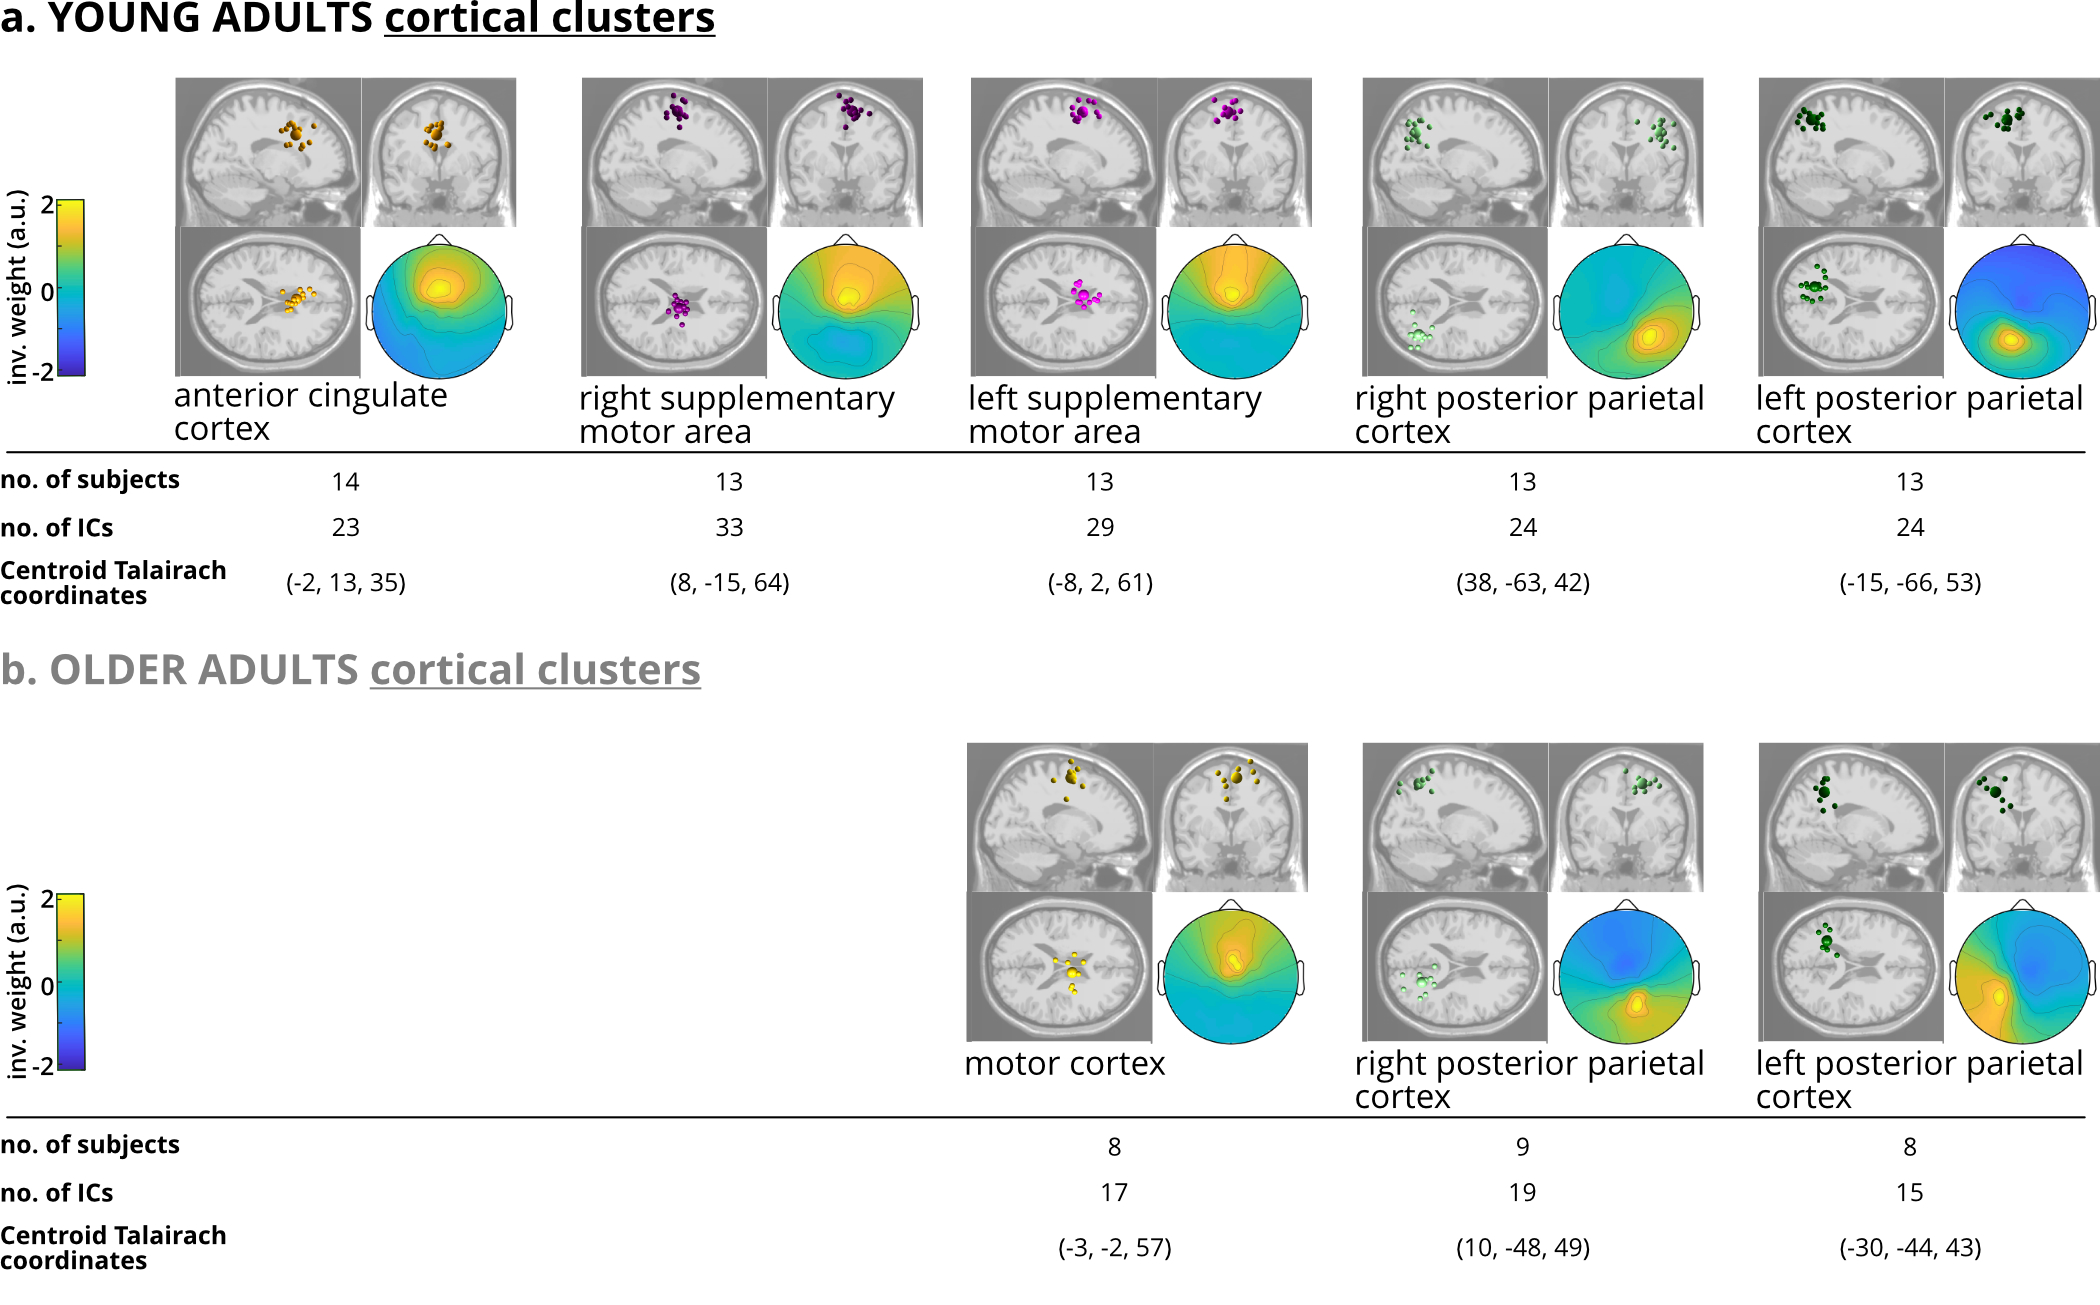
\includegraphics[width=\linewidth]{../img/figure 2 - individual cluster.jpg}
    \caption{The location of the group cortical clusters for young and older adults. Older adults did not have an anterior cingulate cortex or differentiated motor cortex cluster.}
    \label{fig:yo_dipoles}
\end{figure}

\begin{figure}[tb]
    \centering
    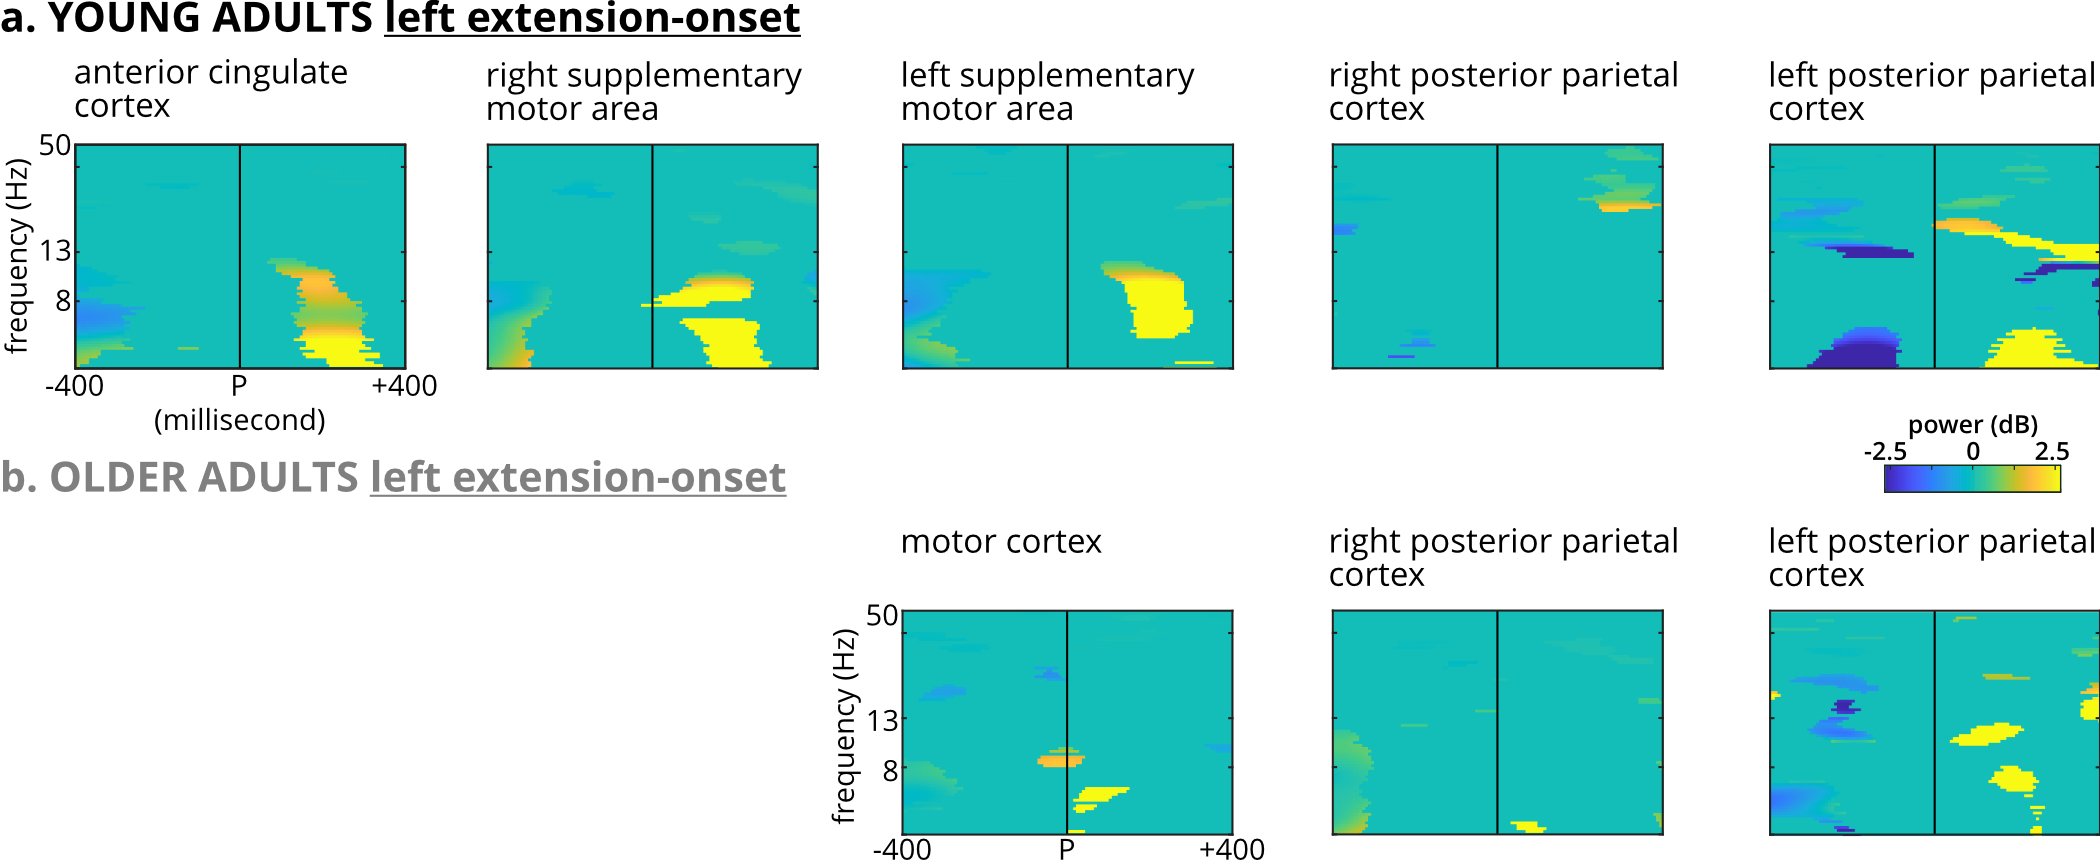
\includegraphics[width=\linewidth]{../img/figure 3 - LEI ERSP.jpg}
    \caption{The spectral fluctuations (ERSP) image around the perturbation even (P) for young and older adults during the \textbf{left extension-onset}. Young adults’ Anterior cingulate cortex, supplementary motor areas, and left posterior parietal cortex had significant theta-band (3-8 Hz) synchronization after the perturbation event. Older adults had minor theta and alpha (3-8 Hz) synchronization in their motor cortex and left posterior parietal cortex.}
    \label{fig:yo_lei}
\end{figure}


\begin{figure}[tb]
    \centering
    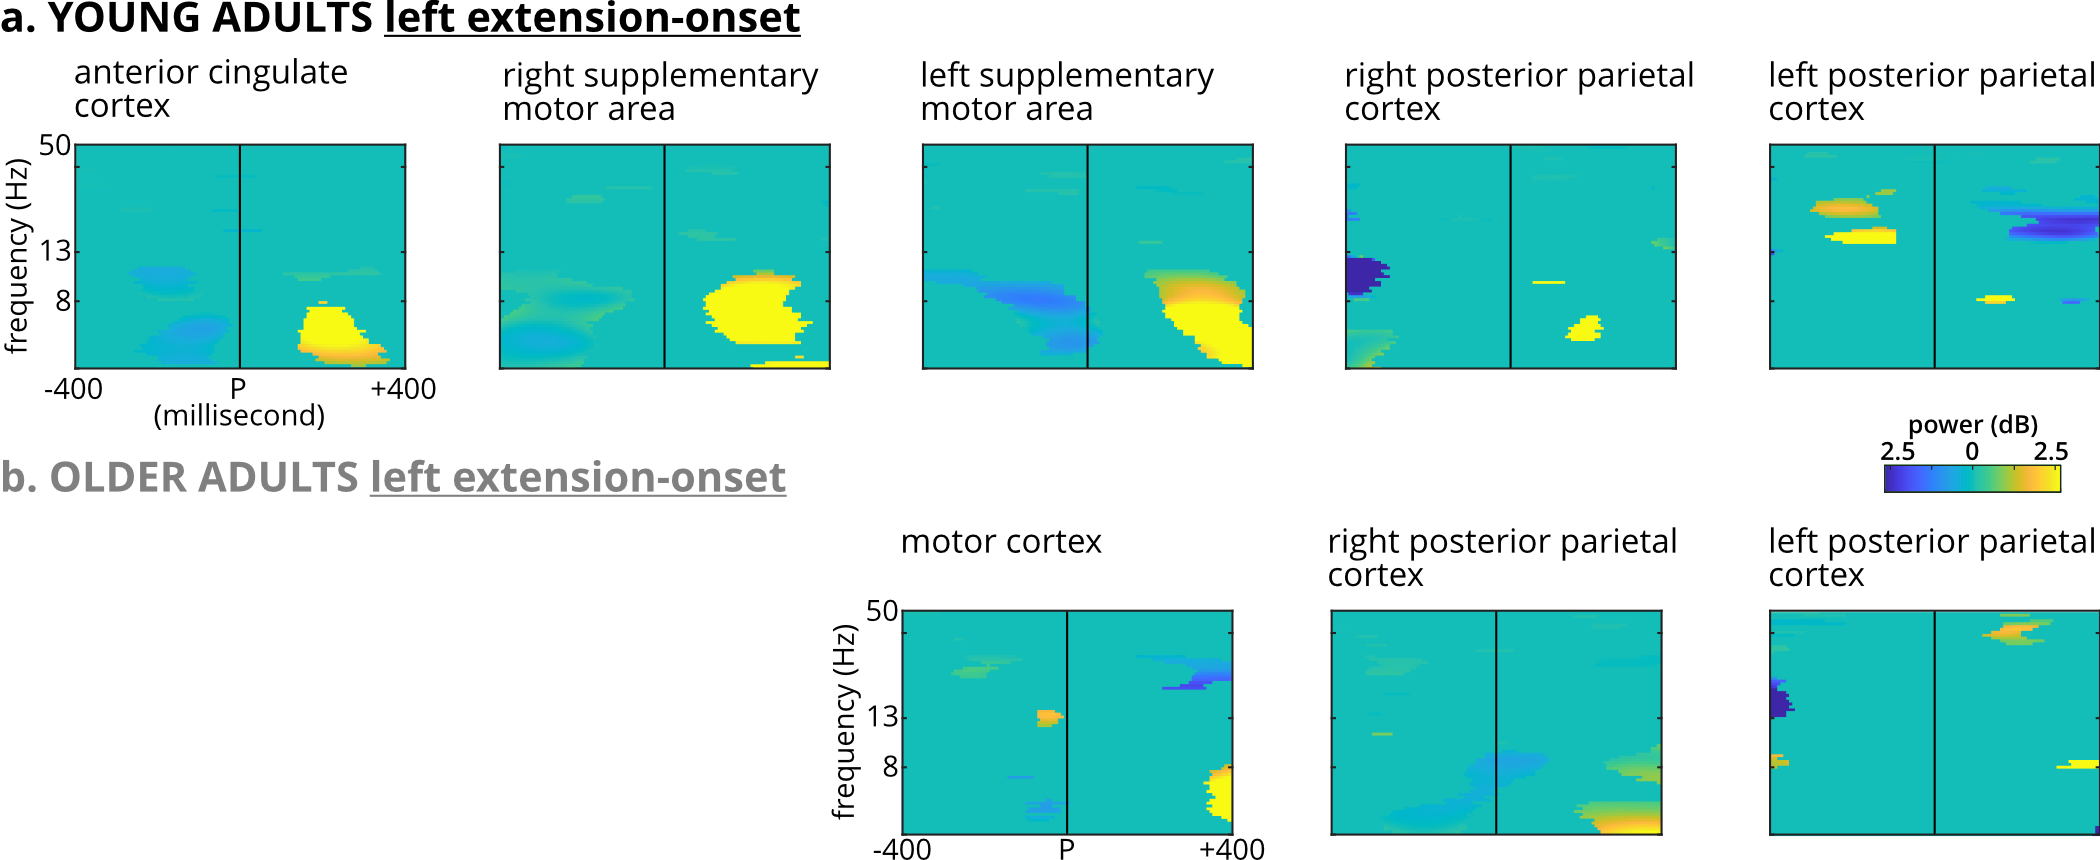
\includegraphics[width=\linewidth]{../img/figure 4 - LME ERSP.jpg}
    \caption{The spectral fluctuations (ERSP) image around the perturbation even (P) for young and older adults during the \textbf{left mid-extension}. Young adults’ Anterior cingulate cortex and supplementary motor areas had significant theta-band (3-8 Hz) synchronization after the perturbation event. Older adults had minor theta and alpha (3-8 Hz) synchronization in their motor cortex and right posterior parietal cortex at +400ms.}
    \label{fig:yo_lme}
\end{figure}

\section{Results}
Young adults’ EEG resulted in more individual “brain” ICs and more group-level clusters than older adults (Figure \ref{fig:yo_dipoles}). The median “brain” component for young adults was 22 per subject, which was significantly greater than the 10 per subject median for older adults (Wilcoxon rank-sum test, p< 0.0005). Young adults had five clusters with ICs from> 70\% of the subjects. The clusters were at the anterior cingulate cortex, right supplementary motor area, left supplementary motor area, right posterior parietal cortex, and left posterior parietal cortex. Older adults had only three clusters with ICs from > 70\% of the subjects. Since the ICs within the clusters were more spread to assign a Broadmann area to the clusters, only the general cortical area was attributed to the older adult clusters. The clusters were at the motor cortex, left posterior parietal cortex, and right posterior parietal cortex.

Young adults had strong theta-band (3-8Hz) synchronization locked to the perturbations in the anterior cingulate and supplementary motor areas for both left extension-onset. However, older adults only showed slight theta synchronization after the perturbations in the motor cortex (Figure \ref{fig:yo_lei}a). The left posterior parietal cortex had increased theta and alpha synchronization for both young and older adults after the perturbation event. However, the right posterior parietal cortex did not show significant spectral fluctuations locked to the perturbation in either young and older adults (Figure \ref{fig:yo_lei}a,b). Both young and older adults also demonstrated theta-alpha desynchronization before the perturbation event in the left posterior parietal cortex.

Mid-extension perturbations also elicited theta-band synchronization in the young adults’ anterior cingulate and right and left supplementary motor areas (Figure \ref{fig:yo_lme}a). Older adults, however, only had slight theta-band motor cortex synchronization toward the end of the 400 ms window (Figure \ref{fig:yo_lme}b). The left posterior parietal cluster had a beta-band (13-35 Hz) synchronization before perturbation which was followed by a beta desynchronization after the perturbations. Older adults did not show significant posterior parietal spectral fluctuations before or after the perturbation event.

Brain to muscle connectivity analysis showed selective anterior cingulate causal muscle relations in young adults and the left parietal cortex causal relation to all muscles for older adults (Figure \ref{fig:b2m}).  The anterior cingulate elicited left soleus activity after the perturbations in the left extension-onset perturbations but mostly elicited the left posterior deltoid for left mid-extension perturbations (Figure \ref{fig:b2m}a,b). The right supplementary motor area had a consistent causal connection to all left-side muscles after the perturbation event for young adults. Compared to the left mid-extension, the left supplementary motor area and right posterior parietal cortex seem to elicit more activity in the anterior and posterior deltoid during left extension-onset perturbations.  The motor cortex and the left posterior parietal cortex of the older adults elicited muscular activity to all left-side muscles (Figure \ref{fig:b2m}c,d). The older adults’ right posterior parietal cortex seemed to have stronger causal connections to the soleus and rectus femoris for left extension onset and to the posterior deltoid for the left mid-extension perturbations.

The lower-limb muscles had an increasing causal relationship to the anterior cingulate activity in young adults, and most older adults’ muscles had an increasing causal relation to the motor cortex during and around the perturbations (Figure \ref{fig:m2b}). The left-side tibialis anterior, soleus, and rectus femoris had increased connectivity to the anterior cingulate cortex around the left extension-onset perturbations. On the other hand, only the left rectus femoris had strong increasing connectivity to the anterior cingulate after left mid-extension perturbations. The left and right supplementary motor areas had increased connectivity from the anterior deltoid in the left-extension-onset, but the left rectus femoris was the common, increasing connectivity for the left and right supplementary motor areas for the mid-extension perturbations. Interestingly, the anterior deltoid connectivity to the right supplementary motor area decreased after the left mid-extension perturbations. All muscles had increased causal relation to the older adults' motor cortex during and after the left mid-extension perturbations (Figure \ref{fig:m2b}c). However, the mid-extension perturbations did not increase left tibialis anterior and posterior deltoid connectivity to the motor cortex (Figure \ref{fig:m2b}d). All the left-side muscles also had increased connectivity to the left or right posterior parietal cortex for older adults.

\section{Discussion}
We quantified the electrocortical spectral dynamics and corticomuscular connectivity around perturbations during recumbent stepping for young and older adults. Young adults had concentrated electrocortical sources in the anterior cingulate, left and right supplementary motor area, and left and right posterior parietal cortex. The anterior cingulate and supplementary motor area clusters consistently showed strong theta-band synchronization after the perturbation event. Older adults, however, had fewer electrocortical sources, especially in the anterior cingulate cortex and supplementary motor area region. Also, older adults only showed slight significant synchronization after the perturbations compared to unperturbed stepping, suggesting that the older adults’ electrocortical activity was not significantly different from the unperturbed stepping. Directional causal connectivity results showed a subset of muscles were directly influenced by the anterior cingulate activity, and only a subset of muscles  had a direct influence on the anterior cingulate activity. Interestingly, older adults increased their corticomuscular connectivity after the perturbation event and had consistent left posterior parietal to muscle connectivity during extension-onset and mid-extension perturbations. The results  provide more evidence of significant corticomuscular connectivity despite the plateaued cortical activity for older adults.

\begin{figure}[H]

    \centering
    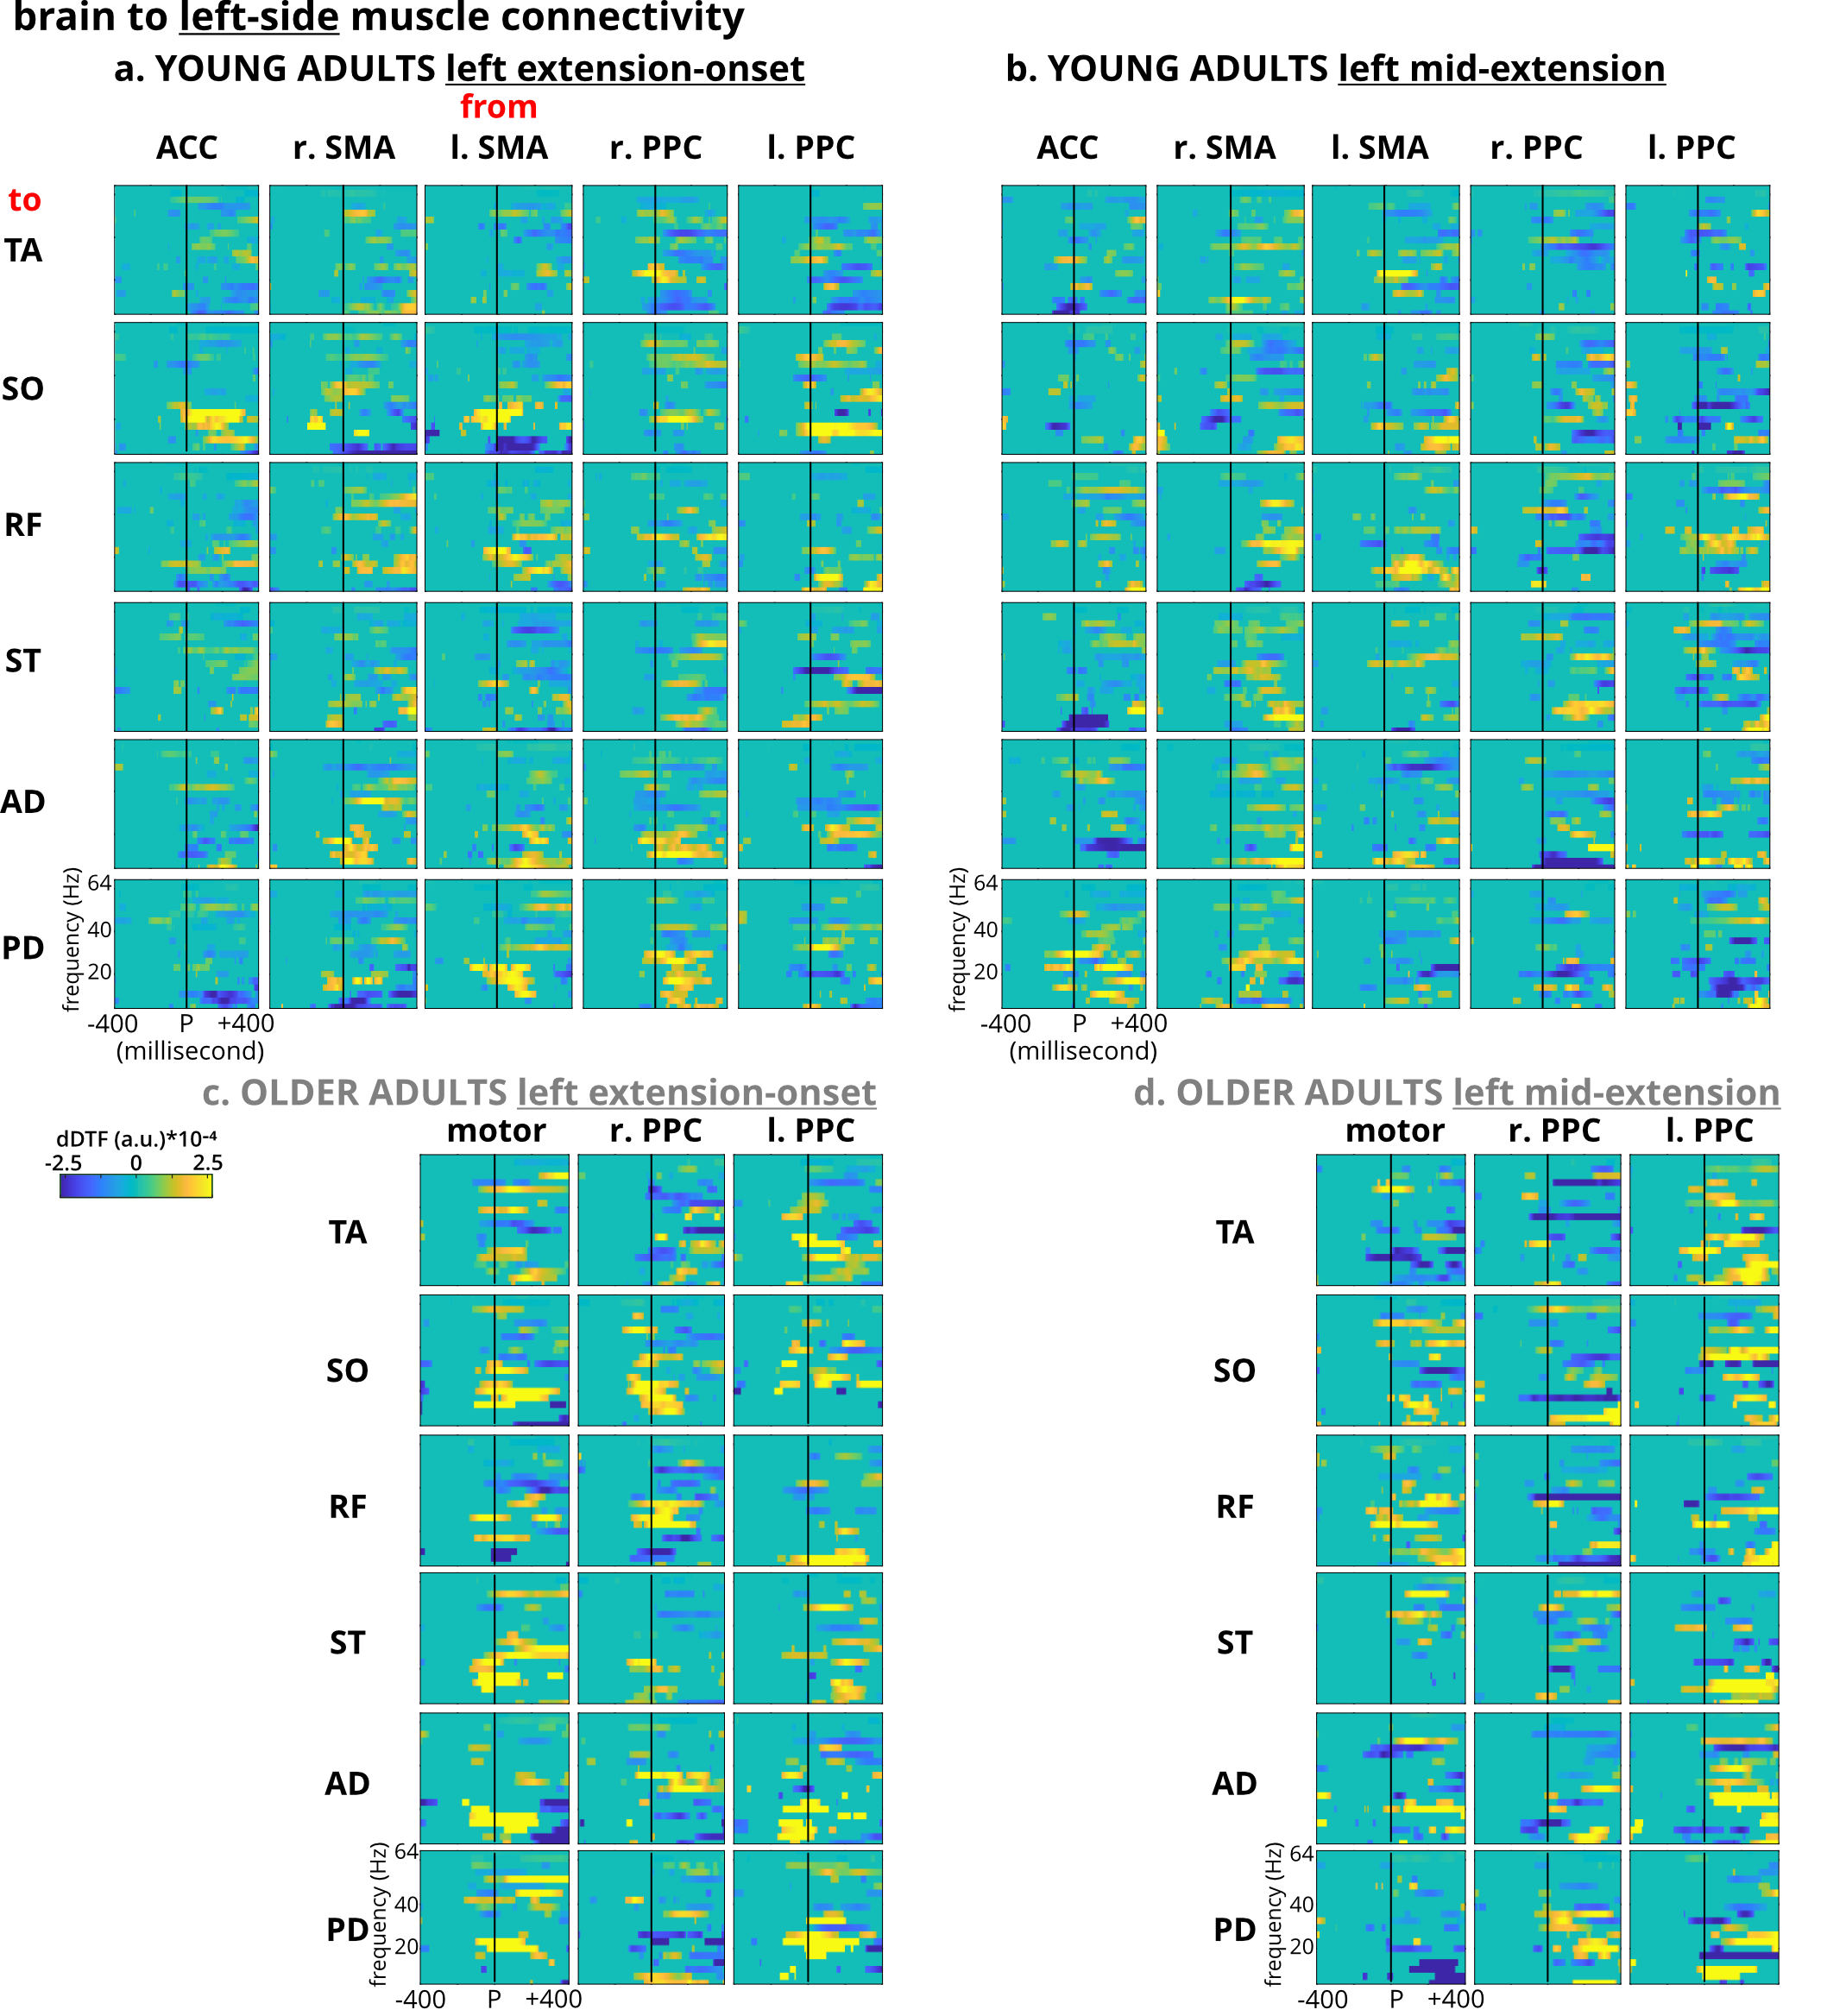
\includegraphics[scale=0.85]{../img/figure 5 - B2M connectivity.jpg}
    \caption{Brain to muscle connectivity. Young adults’ Anterior cingulate cortex had strong causal relation with the left soleus in the left extension-onset and with posterior deltoid in the left mid-extension. Older adults had consistent casual relation from the motor cortex to most of the left-side muscles during both tasks. The left posterior parietal cortex had strong connectivity to older adults’ muscles in both tasks. ACC = Anterior cingulate cortex, r. \& l. SMA = right and left supplementary motor area, r. \& l. PPC = right and left posterior parietal cortex, TA = tibialis anterior, SO = soleus, RF = Rectus femoris, ST = semitendinosus, AD = anterior deltoid, PD = posterior deltoid.}
    \label{fig:b2m}
\end{figure}

Older adults had fewer electrocortical ICs per subject and fewer cortical group clusters than young adults. Previous neuroimaging studies have suggested overactivation of the brain areas in older adults for performing a similar motor task as young adults \cite{Reuter-Lorenz2008-bn}. Such overactivity results in several brain regions becoming active, likely with similar signal characteristics \cite{Seidler2010-yv}. The activity of the overactive regions may not be temporally independent, resulting in shared ICs for different regions, which in turn, would be rejected by DIPFIT algorithm because one of the basic assumptions of the inverse solution is that the brain ICs are dipolar. Further, activity synchrony of different regions of the brain would create a global signal pattern that, with common average referencing, would be canceled from the signal during preprocessing \cite{Roeder2020-tv,Chella2016-zf}.

Young adults had selective information flow to and from the anterior cingulate, but older adults did not present anterior cingulate activity with the presence of the perturbations. The anterior cingulate cortex compares the expected motor goals with the sensory inputs \cite{Holroyd2002-fl,Shenhav2013-qj}, so we hypothesized that part of the sensory input would come from a subset of muscles. We found that during extension-onset tibialis anterior, soleus, and rectus femoris elicit anterior cingulate activity, while during mid-extension perturbations, recuts femoris has the most significant connectivity to the anterior cingulate (Figure \ref{fig:m2b}a,b). Interestingly, upper limb muscles (left anterior deltoid and posterior deltoid) did not contribute to the anterior cingulate activity. Older adults, however, lacked a group cluster located at the anterior cingulate cortex. Looking at our previous research on muscular co-contraction in the previous chapter, both young and older adults generally used their lower-limb muscles to drive the stepper during the perturbed step. So, the lack of anterior cingulate response in older adults might be beyond the lack of sensory input.

\begin{figure}[!h]

    \centering
    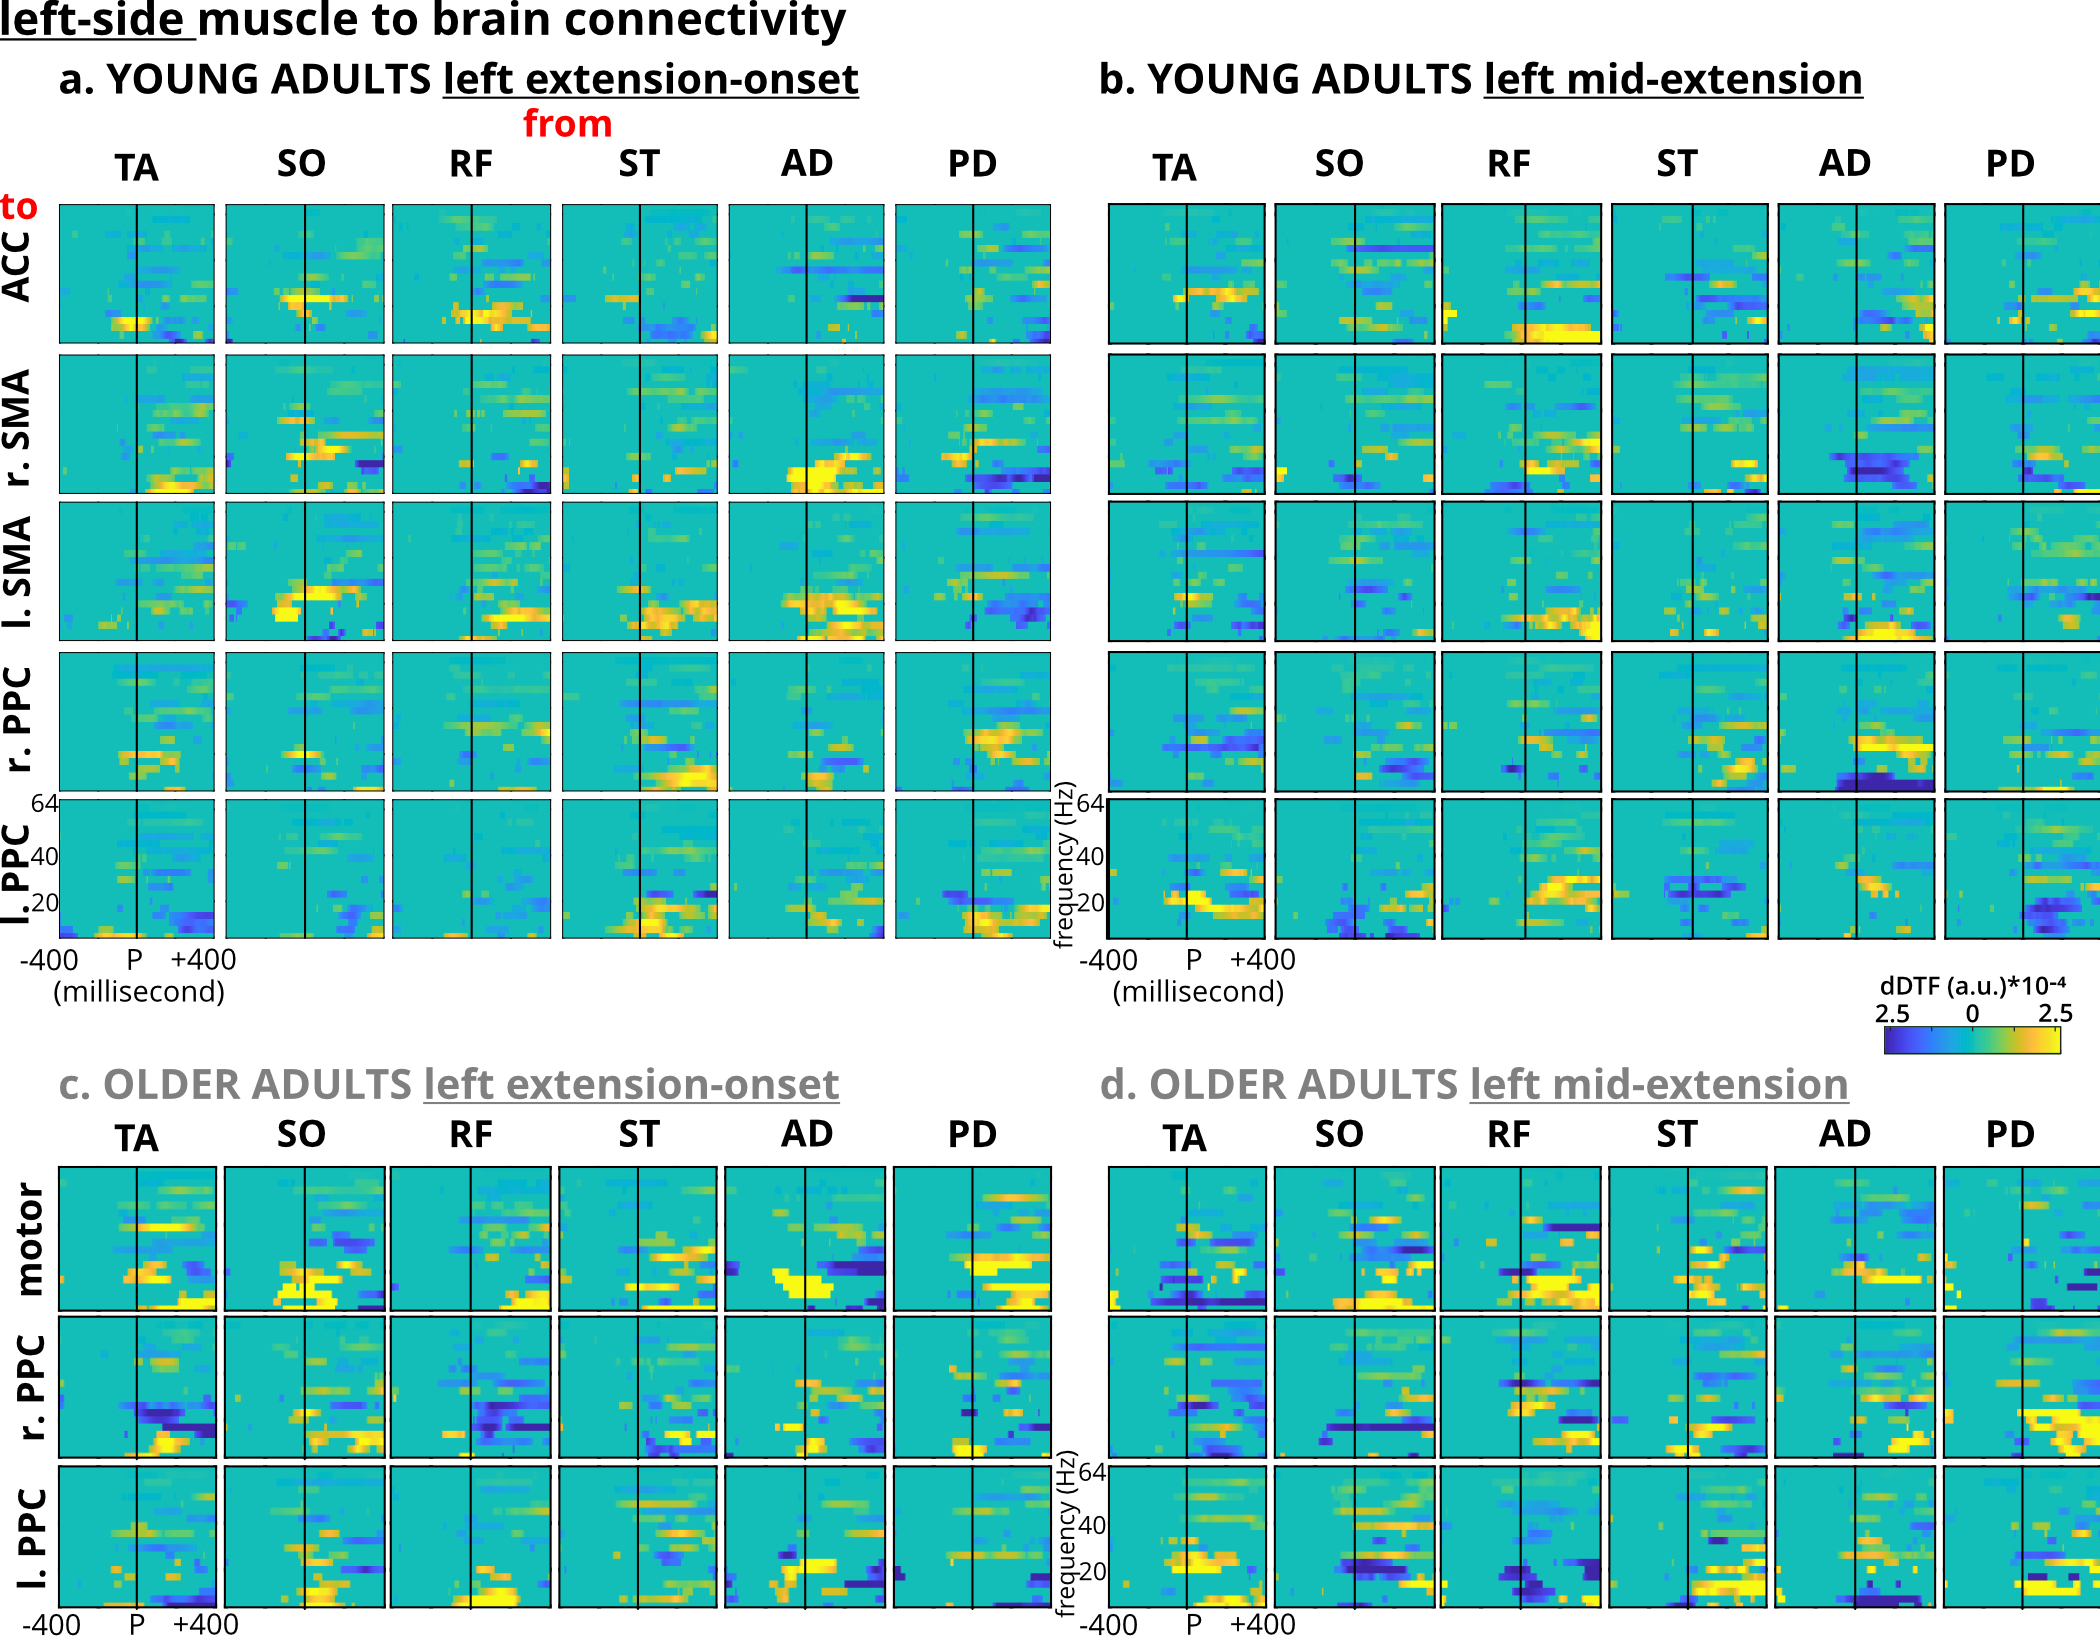
\includegraphics[width=\linewidth]{../img/figure 6 - M2B connectivity.jpg}
    \caption{Muscle to brain connectivity. Young adults’ lower-limb muscles had causal relations to the anterior cingulate cortex. Older adults had consistent casual relation from the muscles to motor cortex. TA = tibialis anterior, SO = soleus, RF = Rectus femoris, ST = semitendinosus, AD = anterior deltoid, PD = posterior deltoid, ACC = Anterior cingulate cortex, r. \& l. SMA = right and left supplementary m0tor area, r. \& l. PPC = right and left posterior parietal cortex.}
    \label{fig:m2b}
\end{figure}

Older adults still maintained corticomuscular connectivity despite fewer cortical areas involved in the process. The left posterior partial connectivity to muscles seemed stronger for older adults. While older adults had only one overall cortical cluster at the motor cortex, almost all left-side muscles seem to have strong bi-directional connectivity with that cluster (Figure \ref{fig:b2m}c,d and Figure \ref{fig:m2b}c,d). This strong connectivity is in line with the previous studies indicating increased corticomuscular connectivity for challenging motor tasks, especially from the motor cortex \cite{Johnson2012-fv,Kamp2013-ga}. Interestingly, the left posterior parietal cortex had a stronger causal relation to older adults’ muscles across both left mid-extension and extension-onset tasks than young adults. Studies with stroke patients had previously indicated the role that the left posterior parietal cortex has in joint impedance control during perturbed upper limb tasks \cite{Mutha2014-ea,Mutha2012-ep}. The more active left posterior partial connectivity and subsequently impedance control in older adults might explain why older adults used fewer muscle pairs to drive the stepper (i.e., older adults had fewer muscle-pairs with agonist-dominant response).

Limitations of this study include a low number of unperturbed strides and a lack of cross-frequency coherence analysis. Despite acceptable temporal and frequency resolution, dDTF apparently requires many trials, at least more than 100 trials, to yield to acceptable results based on previous locomotor studies \cite{Artoni2017-it,Peterson2019-wz}. There were \td30 catch strides in our study and \td50-60 strides during either the pre or post blocks. These limited strides were insufficient for the dDTF connectivity analyses. Alternative connectivity methods such as wavelet analyses may be better suited to analyze lower numbers of trials. The majority of our young adults’ motor cortex responses were at the theta-band, while the muscular activity had high beta and gamma (20+Hz) frequency activities. This disparity in frequency response might skew dDTF and similar connectivity approaches, which by design look for a causal relation between signals in a similar frequency range \cite{Korzeniewska2003-ol}. Also, the 4Hz-frequency resolution determined by the dDTF results in just two data points for the theta-band (3-8 Hz) connectivity. Treating different frequency bands as separate signals and fitting multivariate autoregressive models with different orders might result in a stronger representation of theta-band responses in the connectivity analysis.

Overall, the stepping perturbations increased bi-directional corticomuscular connectivity in  young and older adults. Despite finding fewer cortical clusters for the older adults, all muscles had a significant causal relation to the motor left posterior parietal cortices; the posterior parietal cortex is responsible for joint impedance control, suggesting that impedance control might be a stronger motor control paradigm for older adults. The results provide new evidence that modifying perturbation timing can change connectivity and enhance specific corticomuscular pathways. Such corticomuscualr enhancments can be benficial in providing closed-loop and personalized rehabilitation \cite{Reinkensmeyer2016-ip}.

\bibliographystyle{ieeetr}
\bibliography{../refs}
% \printbibliography
\end{document}